% chktex-file 3 chktex-file 18 chktex-file 36

\section*{Exercise 3.}

\textbf{Nocedal \& Wright: Ex 3.1 }

Program the steepest descent and Newton algorithms using the backtracking line search, Algorithm 3.1. Use them to minimize the Rosenbrock function (2.22). Set the initial step length $\alpha = 1$ and print the step length used by each method at each iteration. First try the initial point $x_0 = (1.2,1.2)^T$ and then the more difficult starting point $x_0 = (-1.2, 1)^T$.

\textbf{Solution:}

The following packages are going to be used in this exercise:

\begin{minted}{python}
    import numpy as np
    import sympy as sp
    import matplotlib.pyplot as plt
    from sympy.tensor.array import derive_by_array
    from numpy.linalg import inv, norm  
\end{minted}

The package \mintinline{python}{numpy} is for the management of arrays, matrices and linear algebra. The package \mintinline{python}{sympy} is used in the calculation of the symbolic derivatives of $f$. The package \mintinline{python}{matplotlib.pyplot} is for the final comparison graphs. In the following steps I'm going to define the function and automatically calculate its derivatives.

\[ f(x,y) = 100(y-x^2)^2 + (1-x)^2 \]

\begin{minted}{python}
    dim = 2
    x = sp.symbols("".join([f"x_{i+1} " for i in range(dim) ])[:-1])
    f = lambda x : 100*(x[1]-x[0]**2)**2 + (1-x[0])**2
    D = lambda expr: derive_by_array(expr,x)
    Df = sp.lambdify([x],D(f(x)))
    Hf = sp.lambdify([x],D(D(f(x))))
\end{minted}

Now, for the algorithm. We choose $x_0$ before starting the process. Then,
\[ \everymath{\displaystyle}
\arraycolsep=1.8pt\def\arraystretch{1.5}
\begin{array}{rclcrcl}
    f_k & = & f(x_k), & \hspace{1em}  & Df_k & = & Df(x_k),\\
    p_k & = & -B_k^{-1} Df_k, & \hspace{1em}  & x_{k+1} & = & x_{k} + \alpha_k p_k,
\end{array} \]
where $B_k = Hf(x_k)$ in Newton's method and $B_k = I$ in the steepest descent method. $\alpha_k$ is chosen according to the backtracking method,
\[ \alpha_k = \max\left\{ \rho^m \alpha \;:\; f(x_k + \rho^m \alpha p_k ) < f(x_k) + \gamma \rho^m Df(x_k)^T p_k \right\}. \]
This is the code corresponding to the backtracking method,

\begin{minted}{python}
    def backtracking(alpha, gamma, rho, x_k, f_k, Df_k, p_k):
    alpha_k = alpha
    backtracking = f(x_k + alpha_k*p_k) - (f_k + gamma*alpha_k*Df_k.T @ p_k)
    while backtracking > 0 :
        alpha_k = alpha_k * rho
        backtracking = f(x_k + alpha_k*p_k) - (f_k + gamma*alpha_k*Df_k.T @ p_k)
    return alpha_k
\end{minted}

Also, for the Newton's method and steepest descent, the code is the following

\begin{minted}{python}
    def newton(alpha, gamma, rho, n, x_0, f, Df, Hf):
        x_k = x_0
        x_list = [x_k]
        for i in range(n):
            f_k = f(x_k)
            Df_k = Df(x_k)
            B_k = Hf(x_k)
            p_k = -inv(B_k)@Df_k
            alpha_k = backtracking(alpha, gamma, rho, x_k, f_k, Df_k, p_k)
            x_k = x_k+alpha_k*p_k
            x_list.append(x_k)
            if norm(Df_k) < epsilon:
                break
        return x_list

    def gradient_descent(alpha, gamma, rho, n, x_0, f, Df, Hf):
        x_k = x_0
        x_list = [x_k]
        for i in range(n):
            f_k = f(x_k)
            Df_k = Df(x_k)
            p_k = -Df_k
            alpha_k = backtracking(alpha, gamma, rho, x_k, f_k, Df_k, p_k)
            x_k = x_k+alpha_k*p_k
            x_list.append(x_k)
            if norm(Df_k) < epsilon:
                break
        
        return x_list
\end{minted}

The parameters I'm going to use in the algorithm are defined as follows,
\begin{minted}{python}
    epsilon = 1e-12
    n= 2000
    alpha = 1
    rho = 0.94
    gamma = 0.6
    x_0 = np.array([1.2,1.2])
\end{minted}
$\varepsilon =$ \mintinline{python}{epsilon} is the termination criterion number for which the algorithm stops when $\|Df(x_k)\| < \varepsilon$. $n =$ \mintinline{python}{n} is the maximum number of iterations I want for the algorithm. $(\alpha, \rho, \gamma) =$ \mintinline{python}{(alpha, rho, gamma)} are the parameters for the backtracking line search and $x_0 = $ \mintinline{python}{x_0} is the initial position. The results are the following for $x_0 = (1.2,1.2)$ and $x_0 = (-1.2, 1.0)$ respectively.
\begin{figure}[h]
    \centering
    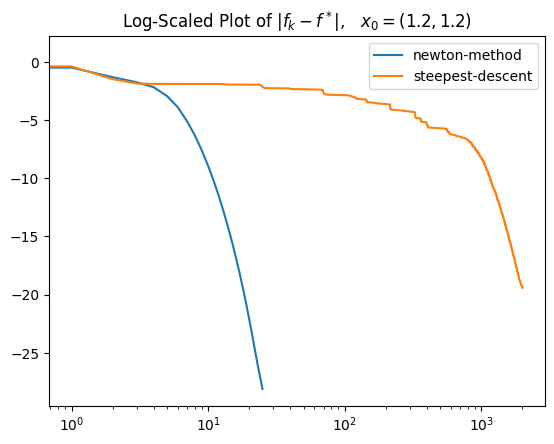
\includegraphics[width=0.45\textwidth]{../pictures/hw2ex3.1.png}
    \hfill
    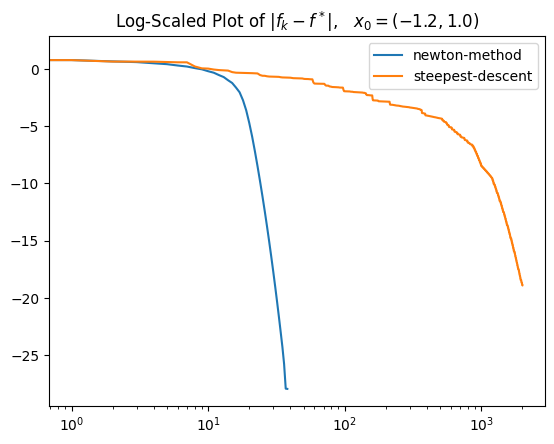
\includegraphics[width=0.45\textwidth]{../pictures/hw2ex3.2.png}
\end{figure}

Finally, I the step sizes are located in the files \texttt{hw3-newton-stepsizes.txt} and 

\texttt{hw3-steepest-stepsizes.txt} respectively.
